
% submission details
\newcommand{\deadlineOneTime}{noon}
\newcommand{\deadlineOneDate}{16 February 2021}
\newcommand{\submissionOneURL}{https://tabula.warwick.ac.uk/coursework/submission/43213a10-18dc-4e87-8364-c648097af402}
\newcommand{\classroomOneURL}{https://classroom.github.com/a/eQTilEdh}

%\renewcommand{\instructions}{Due at \emph{\deadlineTime} on \emph{\deadlineDate}.}


\cleardoublepage
\chapter{Coursework I}

\section{The Large Arithmetic Collider}

The goal of this coursework is to implement a Haskell program which can solve a challenging combinatorial game that we have named the \emph{large arithmetic collider}. The game focuses on a grid containing mathematical operations. To explain how it works, let us start with a simple example: consider the following row containing the operations \texttt{+31}, \texttt{-26}, \texttt{-14}, and \texttt{-1} from left to right:
\begin{center}
	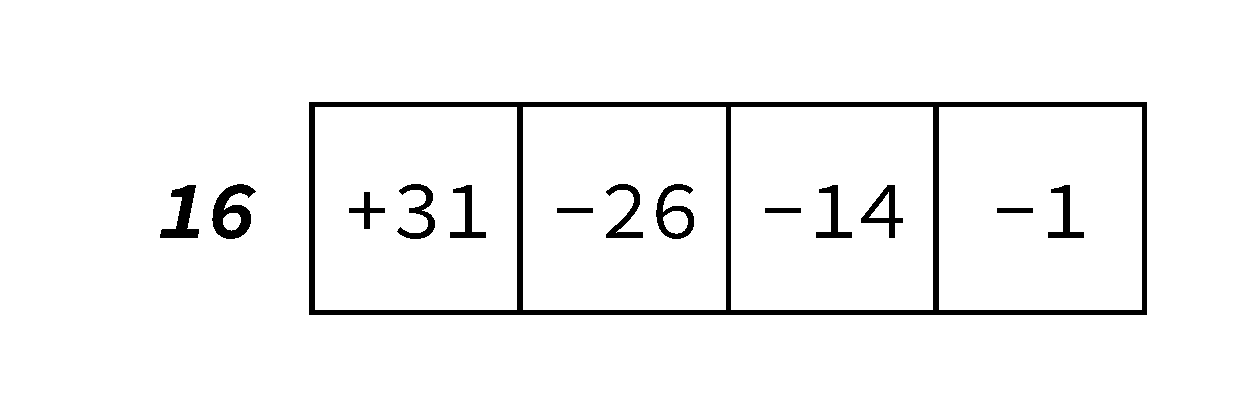
\includegraphics[scale=0.4,trim=0 30 0 30]{cswk/lac1.pdf}
\end{center}
You will also note that this row is annotated with the number $16$ on the left. The goal now is to determine which of the operations contained in the cells result in that number when applied from left to right, starting with $0$. The solution for this example is shown below, where the cells containing operations that can be used to obtain the target number are shaded in grey (we refer to them as ``enabled'' cells):
\begin{center}
	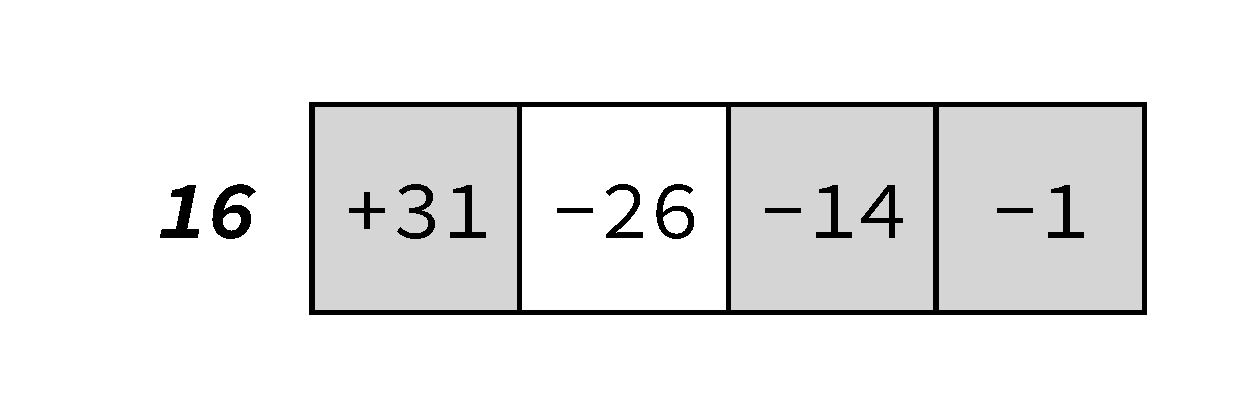
\includegraphics[scale=0.4,trim=0 30 0 30]{cswk/lac1s.pdf}
\end{center}
As we can easily see, this is a solution because $0+31-14-1=16$. Since there are 4 cells in this example and each cell can either be enabled or not, there are $2^4=16$ possible configurations to explore when searching for a solution for this grid. Although there is only one solution for this example, grids may have more than one solution or, indeed, no solution. 

You may notice that we are talking about a ``grid'', but have only shown a single row to illustrate the basic game mechanics. A more realistic grid is shown below:
\begin{center}
	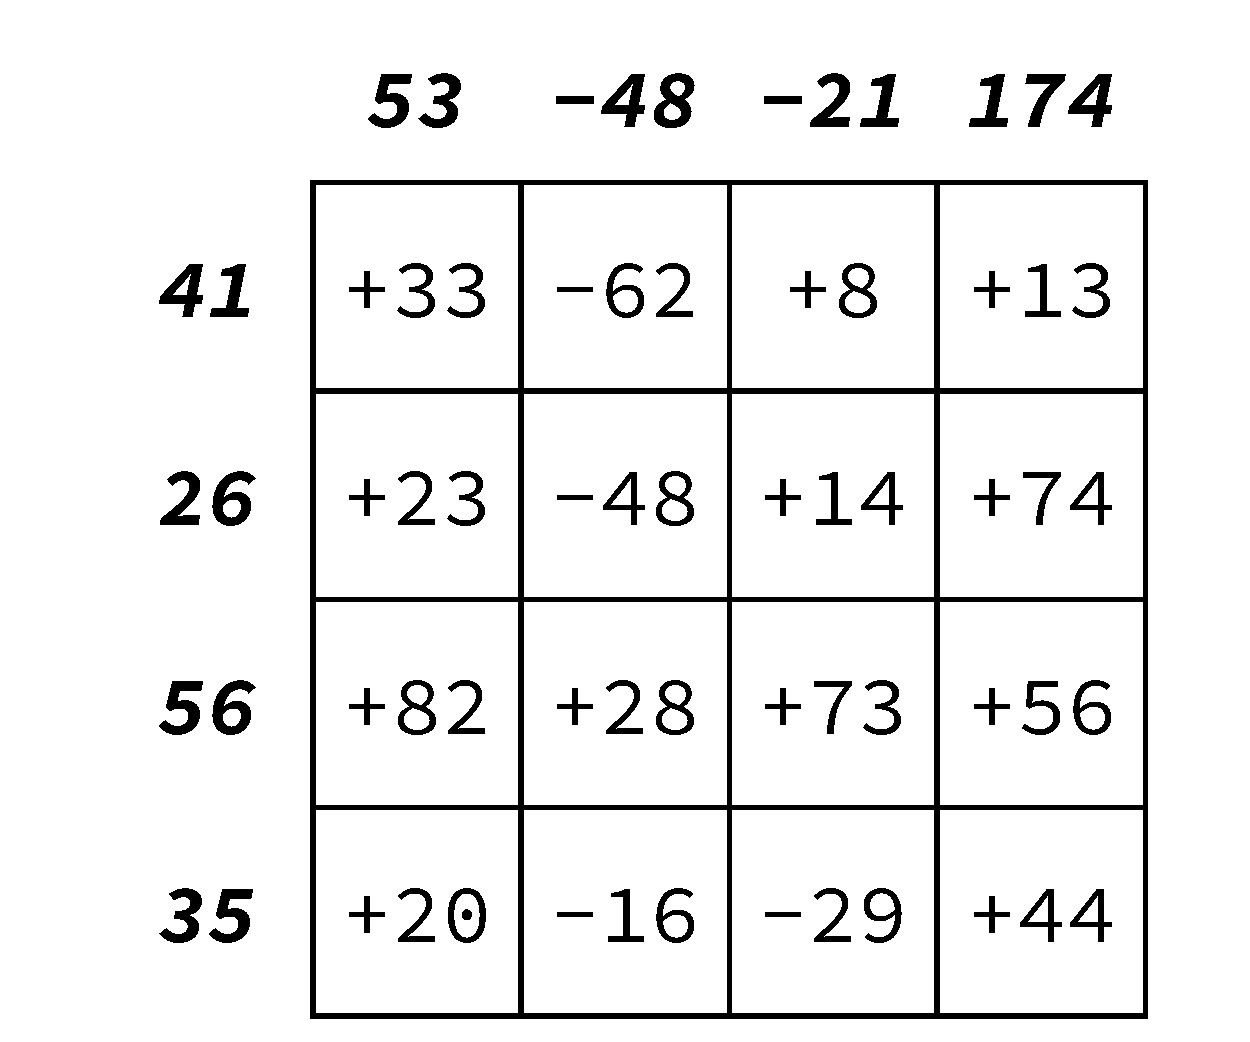
\includegraphics[scale=0.4,trim=0 30 0 30]{cswk/lac2.pdf}
\end{center}
As we can see, every row and every column is annotated with a target number. We must find which operations to enable so that every row results in its target number as described in the previous example and that every column also results in its target number. The rules for columns are the same as for rows: we start with 0 and apply each active operation from top to bottom. The solution for this grid is shown below:
\begin{center}
	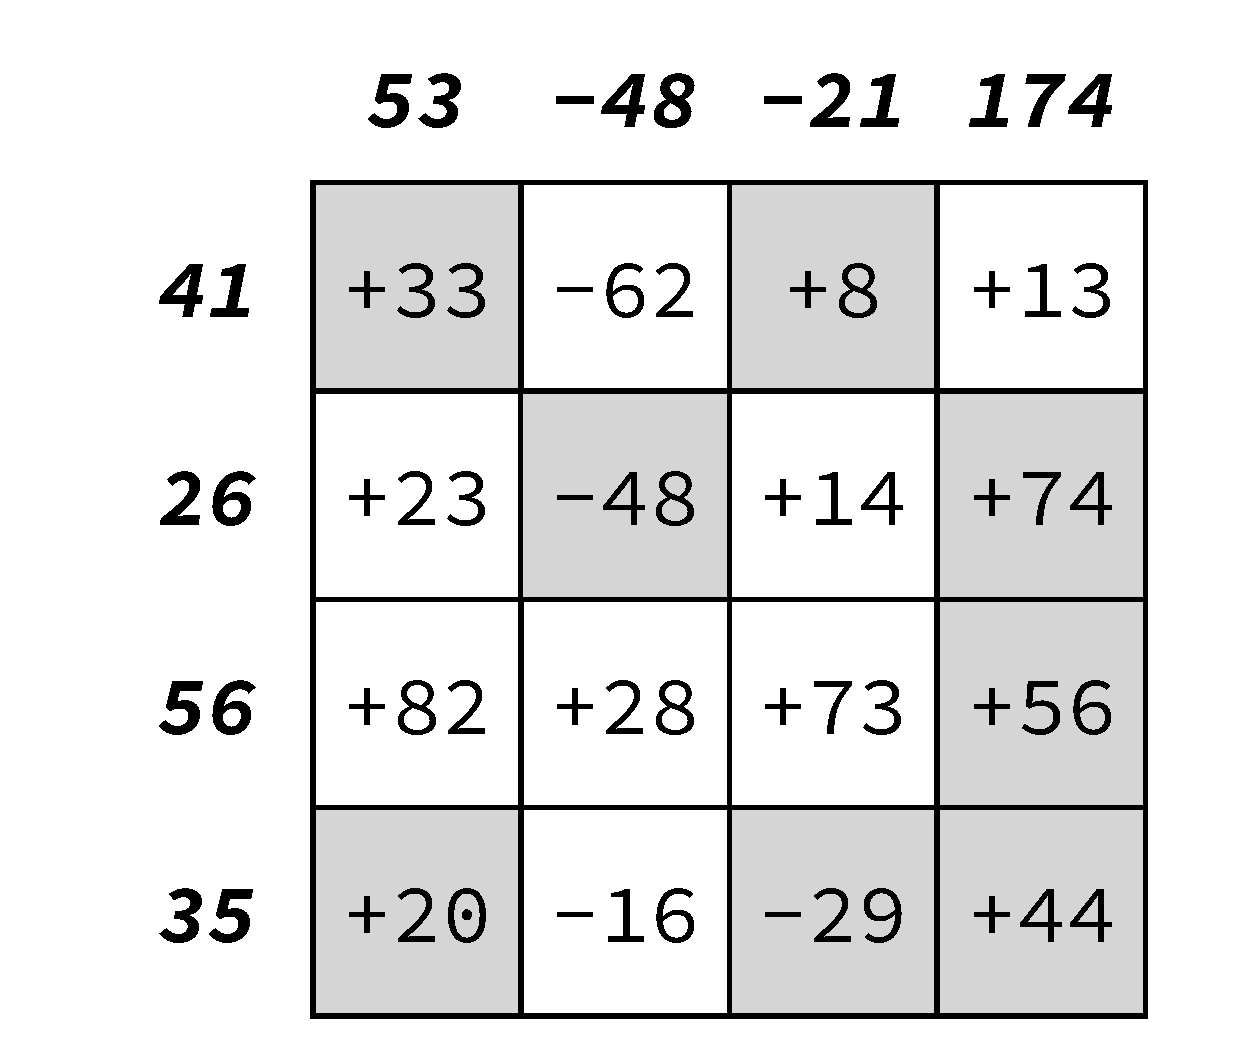
\includegraphics[scale=0.4,trim=0 30 0 30]{cswk/lac2c.pdf}
\end{center} 
Finding a solution for this grid is more difficult. In this example, there are $4 \times 4 = 16$ cells and the number of possible configurations to explore is therefore $2^{16} = 65535$. In general, grids can have arbitrary dimensions and so the number of possible configurations is $2^{\mathit{rows} \times \mathit{columns}}$. Fortunately, such grids are still fairly simple for a computer to solve.

\pagebreak
\subsection{Rotations}

To further increase the difficulty of the game, there is one more game mechanic. While some grids can be solved as they are, we can also consider grids where rows or columns must be \emph{rotated} first. For example, consider the following grid:
\begin{center}
	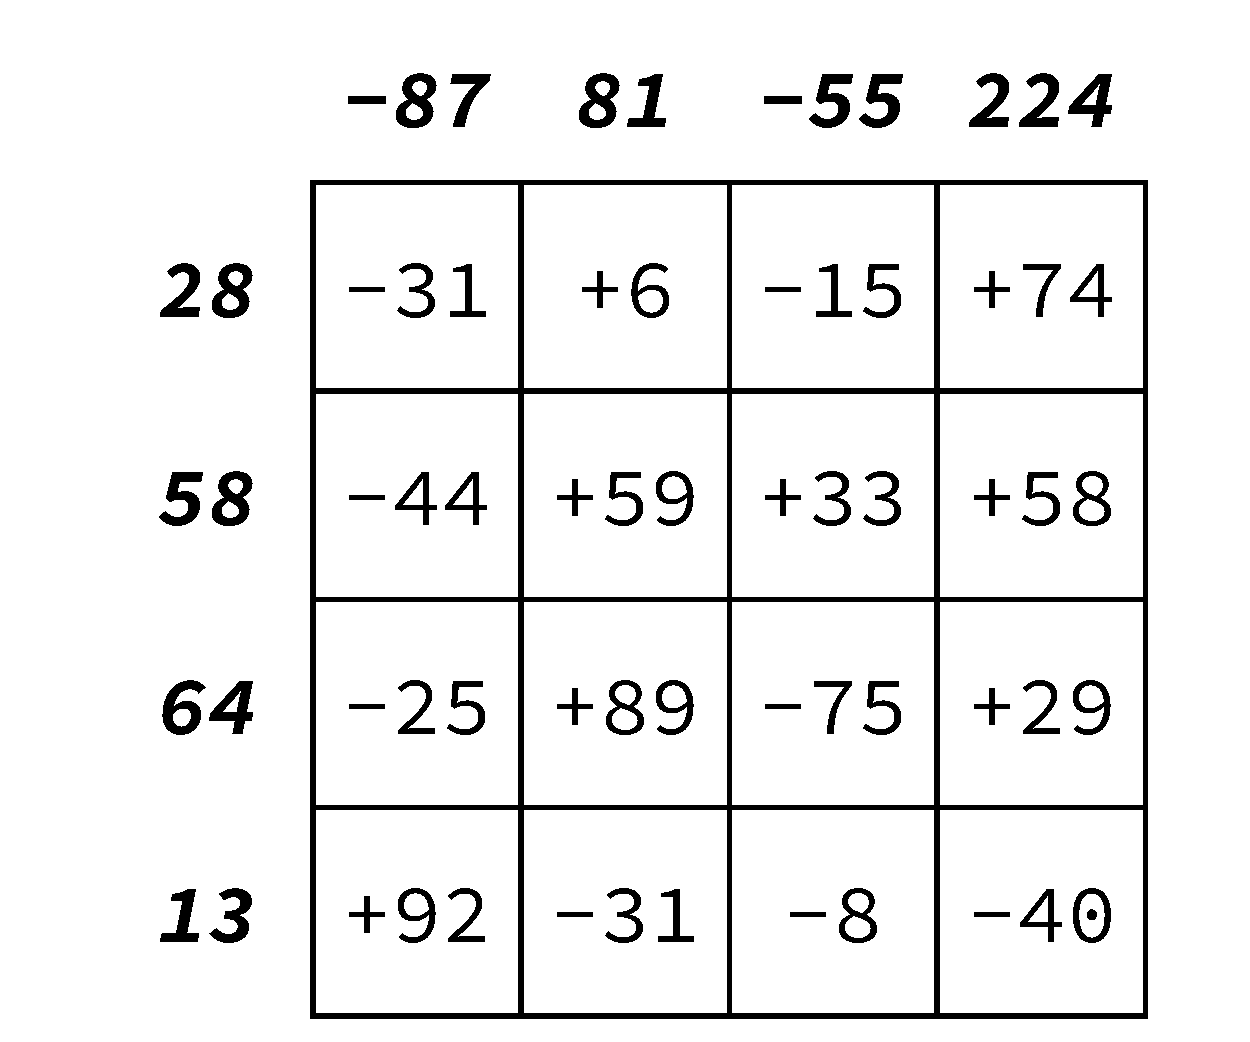
\includegraphics[scale=0.4,trim=0 30 0 30]{cswk/lac3.pdf}
\end{center}
This grid has no solutions as it is. However, we can find solutions if we change the layout of the cells by rotating some of the rows or columns. The rules for this are as follows: we always perform rotations from right to left or bottom to top. Therefore, for a given grid, there are always $\mathit{rows}+\mathit{columns}$ possible rotations. For the example shown above, we can solve it by rotating the last row of the grid:
\begin{center}
	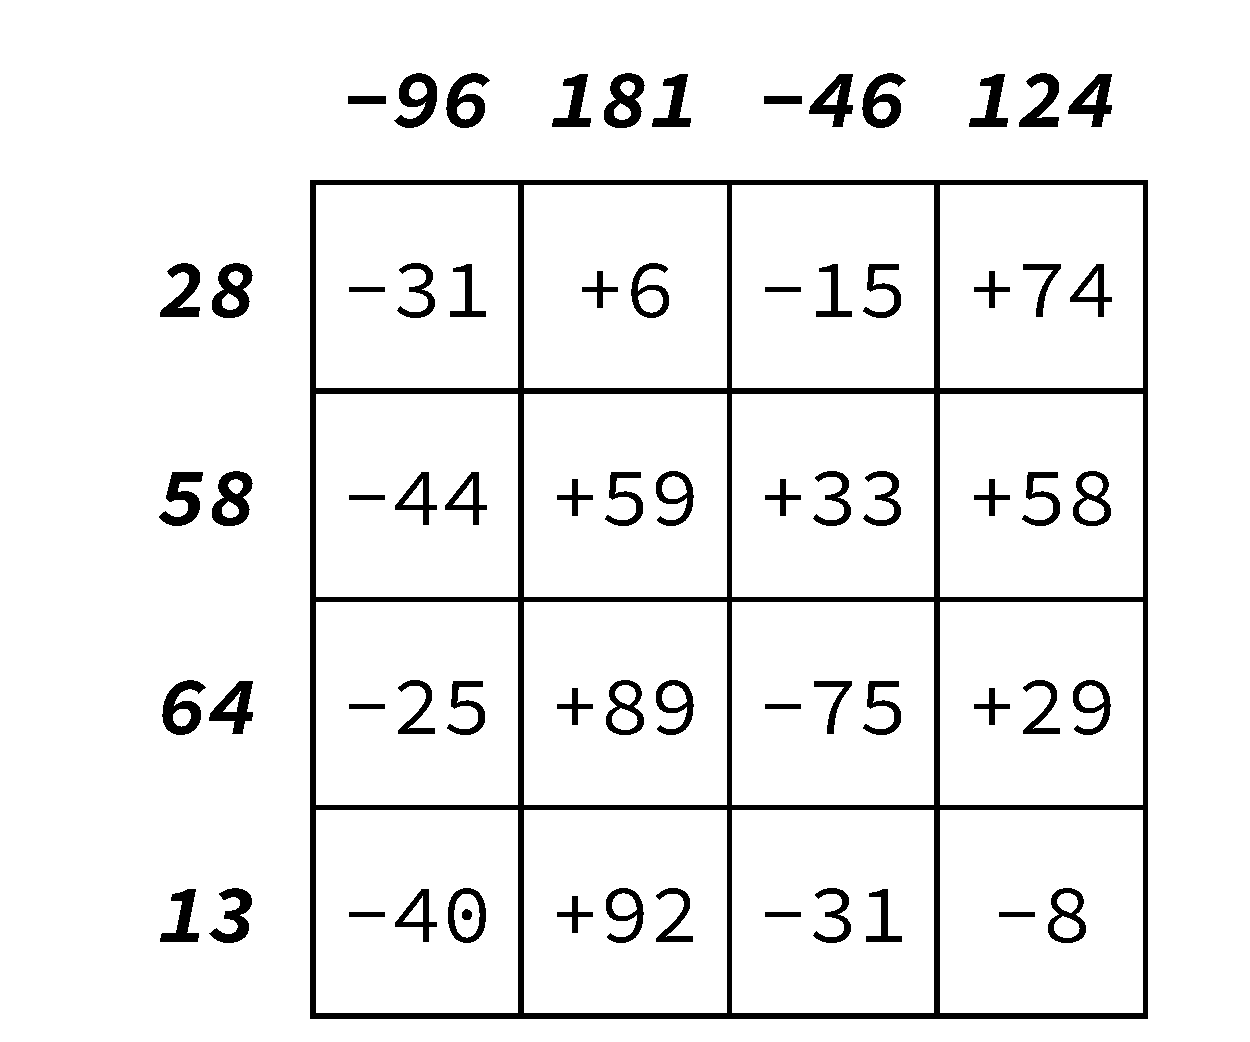
\includegraphics[scale=0.4,trim=0 30 0 30]{cswk/lac3r.pdf}
\end{center}
We refer to applying one such rotation as a \emph{move}. If a grid cannot be solved in zero moves (\emph{i.e.} without rotations), then our goal is to try and solve it in \emph{as few moves as possible}. With the last row rotated as shown above, there is now a solution for the resulting grid:
\begin{center}
	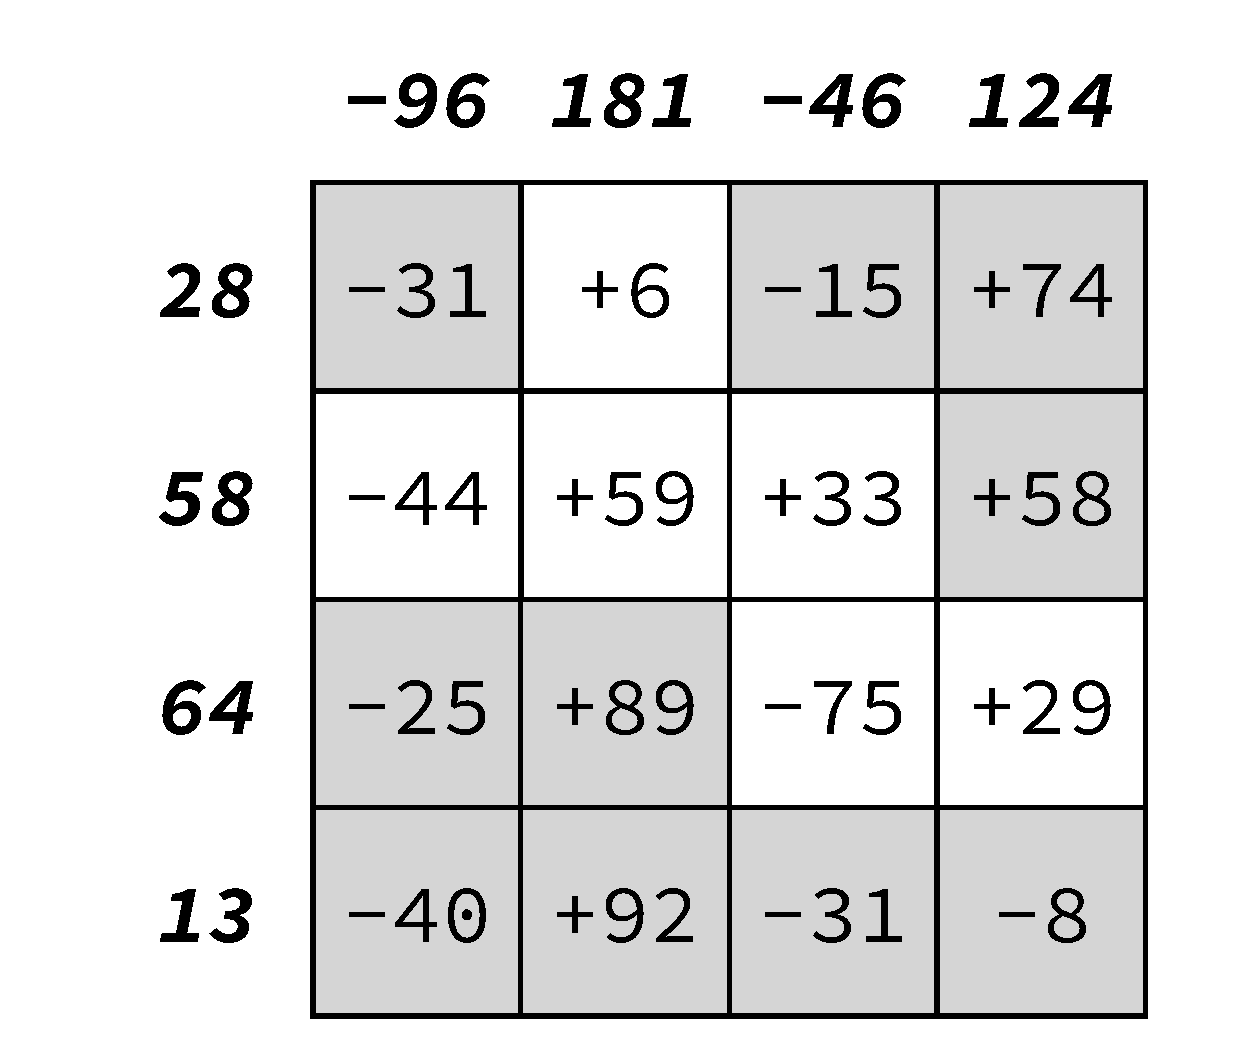
\includegraphics[scale=0.4,trim=0 30 0 30]{cswk/lac3s.pdf}
\end{center}
Finding a solution for a grid that can only be solved with rotations is much harder than finding solutions for one that can be solved in zero moves. In theory, we can use rotations to create an arbitrary arrangement of cells in the grid, thus leaving us with $(\mathit{rows} \times \mathit{columns})!$ many arrangements of cells. That means that for a $4 \times 4$ sized grid such as the one shown above, there are $20,922,789,888,000$ many arrangements of cells. Each cell can then either be enabled or not, so for each of those arrangements there are $2^{4 \times 4}$ possible solutions, leaving us with a total state space of $(4 \times 4)! \times 2^{4 \times 4}$ many possible solutions for a $4 \times 4$ grid. However, fortunately we do not need to search this entire state space since just finding a solution in itself does not tell us how to get there from the grid we start with, so a smarter approach is needed to find a solution in as few moves as possible!

%-----------------------------------------------------------

\section{Before you get started}
\label{sec:cswk1-before-you-start}

Before you get started with this coursework, we \emph{strongly recommend} that you complete all lab exercises up to and including those on data types (\Cref{sec:lab-data-types}). You will find them all extremely helpful in preparing you for the tasks in this coursework!

If you need help while working on the coursework, remember that help is available from me (Michael) and the teaching assistants. I am usually pretty quick to reply to questions, particularly on the Slack. Additionally, see \Cref{sec:useful-resources} for other resources you may find useful.

%-----------------------------------------------------------

\section{Getting started}
\label{sec:cswk1-getting-started}

In order to get started with the coursework, you need to get hold of the skeleton code and ensure that it compiles successfully on your machine. 

\subsection{Obtaining the skeleton code}

There are three different ways in which you can obtain the skeleton code for this coursework. All of them are explained below alongside their various advantages and disadvantages:

\makebox[0.5cm]{\faInfoCircle}~We encourage you to use version control for your work and the first two options below assume you have basic familiarity with version control using \texttt{\small git}. You can read \Cref{sec:git} for a \texttt{\small git} crash course or {\small \url{https://git-scm.com/book/en/v2}} for a more comprehensive introduction.

\paragraph{Option A: Private fork} By following the GitHub Classroom link below, you can create a private fork of our git repository with the skeleton code. This requires a GitHub account, but has the advantage that you have your own private copy of our repository on GitHub that you can write to. That would allow then you to work easily share your work between machines in the labs and at home:
\begin{center}
	\small
	\url{\classroomOneURL}
\end{center}
Once you have accepted the assignment, you can then clone your fork of the skeleton code to your machine with the usual \bashIn{git clone} command where \texttt{\small [username]} is your GitHub username:
\begin{minted}{bash}
$ git clone https://github.com/fpclass/2021-cswk1-[username]
\end{minted}
\paragraph{Option B: Clone} If you do not wish to create a GitHub account or host a copy of your repository there, then you could instead just clone our repository with:
\begin{minted}{bash}
$ git clone https://github.com/fpclass/large-arithmetic-collider
\end{minted}
You will be able to \bashIn{git commit} changes to your local copy of the repository, but you will not be able to \bashIn{git push} them. This is sufficient if you are only planning to work on the coursework from one place (\emph{e.g.} only the lab machines but not your personal computer).

\paragraph{Option C: Archive} If GitHub should be unavailable or you do not have \bashIn{git} installed your machine, you can download a \texttt{\small .zip} file with the skeleton code from the module website.

\subsection{Working with the skeleton code}

You may wish to verify that the code compiles and that all tests fail by entering the \texttt{\small large-arithmetic-collider} directory and running \texttt{\small stack test}:
\begin{minted}{text}
$ cd large-arithmetic-collider
$ stack test
\end{minted}
Running \texttt{\small stack test} will compile your code, run a bunch of unit and property tests on it, and give you a rough indication of how complete your solution is: the more tests pass, the more complete it is. Initially, not all tests will be run (those that are not run will show ``SKIP'' as their status) since they depend on working implementations of other functions. As you make progress with the coursework and complete functions so that they pass their tests, the other tests will then be executed whenever you run \texttt{\small stack test}. %Running \bashIn{stack bench} will run a set of benchmarks on your code. 

You can also use \texttt{\small stack build} to just compile your code and then \texttt{\small stack exec collider} to run the game (or just \texttt{\small stack run} to do both). Note that the game will of course not work properly until you have implemented the tasks for this coursework. Specifically, the first two campaigns will not work until you have implemented the functions up to and including \haskellIn{solve} and the last two campaigns will not work until you have implemented the remaining functions, including \haskellIn{steps}. You can run \texttt{\small stack repl} to load up the REPL, which is useful for debugging.

The skeleton code contains a bunch of files, most of which you do not need to touch. The most important file is \texttt{\small src/Game.hs} which contains the definitions you will need to complete in order to implement the game. There are some definitions to get you started. Firstly, the arithmetic operations that may be contained in cells of the grids are represented as an algebraic data type where each constructor represents one type of operation along with its operand:
\begin{minted}{haskell}
data Action 
  = Add Int 
  | Sub Int 
\end{minted}
Cells themselves are also represented as an algebraic data type comprised of a boolean value indicating whether the cell is enabled or not and an \haskellIn{Action} value representing the arithmetic operation contained in the cell:
\begin{minted}{haskell}
data Cell = MkCell Bool Action
\end{minted}
Rows are comprised of a target number for the row and a list of cells:
\begin{minted}{haskell}
data Row = MkRow Int [Cell]
\end{minted}
Grids are comprised of a list of target numbers for the columns and a list of all the rows in the grid:
\begin{minted}{haskell}
data Grid = MkGrid [Int] [Row]
\end{minted}
Finally, we have a definition for a little helper type to represent directions:
\begin{minted}{haskell}
data Direction = L | R
\end{minted}

%-----------------------------------------------------------

\section{Task}

Complete all definitions in \texttt{\small src/Game.hs} so that the game works as described above. The following function stubs in \texttt{\small src/Game.hs} need to be implemented:

\begin{enumerate}
	\item \haskellIn{eval :: Action -> Int -> Int}\\
	This function should apply an arithmetic operation represented by an \haskellIn{Action} value to an accumulator and return the result. For example, \haskellIn{eval (Add 5) 10} should evaluate to \haskellIn{15}.
	
	\item \haskellIn{apply :: Cell -> Int -> Int}\\
	This function should apply the arithmetic operation contained in a \haskellIn{Cell} value to an accumulator and return the result if the cell is enabled. For example, \haskellIn{apply (MkCell True (Add 5)) 10} should evaluate to a result of \haskellIn{15} while \linebreak \haskellIn{apply (MkCell False (Add 5)) 10} should evaluate to \haskellIn{10}.
	
	\item \haskellIn{result :: [Cell] -> Int}\\
	This function should determine the result of evaluating all the enabled arithmetic operations in a list of cells, starting with $0$. For example, evaluating \haskellIn{result [MkCell True (Add 3), MkCell False (Add 5)]} should result in \haskellIn{3}.

	\item \haskellIn{states :: Cell -> [Cell]}\\
	A function which returns a list with \emph{exactly} two elements that represent the two different states a cell can be in. For example:
	\begin{minted}{haskell}
    states (MkCell False (Add 5))
==> [MkCell True (Add 5), MkCell False (Add 5)]
	\end{minted}

	\item \haskellIn{candidates :: [Cell] -> [[Cell]]}\\
	A function which, given a list of cells in a row, produces all possible combinations of states for those cells. For example:
\begin{minted}{haskell}
    candidates [MkCell False (Add 5), MkCell False (Sub 1)]
==> [ [MkCell False (Add 5), MkCell False (Sub 1)]
    , [MkCell False (Add 5), MkCell True (Sub 1)]
    , [MkCell True (Add 5), MkCell False (Sub 1)]
    , [MkCell True (Add 5), MkCell True (Sub 1)]
    ]
\end{minted}

	\item \haskellIn{solveRow :: Row -> [Row]}\\
	This function should find all solutions for a given row. For example:
\begin{minted}{haskell}
    solveRow (MkRow 4 [ MkCell False (Add 4)
                      , MkCell False (Sub 7)
                      ])
==> [MkRow 4 [MkCell True (Add 4), MkCell False (Sub 7)]]
\end{minted}
	
	\item \haskellIn{solve :: Grid -> [Grid]}\\
	This function should find all solutions for a given grid, without rotating any rows or columns. The cells in the input grid may be in any state. If there are no solutions, an empty list should be returned. For example:
\begin{minted}{haskell}
solve (MkGrid [2,4] [ MkRow 3 [ MkCell False (Add 2)
                              , MkCell False (Add 1)
                              ]
                    , MkRow 3 [ MkCell False (Add 2)
                              , MkCell False (Add 3)
                              ]
                    ])
==> [MkGrid [2,4] [ MkRow 3 [ MkCell True (Add 2)
                            , MkCell True (Add 1)
                            ]
                  , MkRow 3 [ MkCell False (Add 2)
                            , MkCell True (Add 3)
                            ]
                  ]]
\end{minted}

	\item \haskellIn{rotate :: Direction -> [a] -> [a]}\\
	A function which rotates the items in a list to the left or right depending on the specified direction. For example, \haskellIn{rotate L [1,2,3]} should evaluate to \haskellIn{[2,3,1]}. Note that although gameplay will always use rotations to the left (\emph{i.e.} \haskellIn{rotate L}), \haskellIn{rotate R} is required for the tests to work correctly.
	
	\item \haskellIn{rotations :: Grid -> [Grid]}\\
	Given a grid, this function should return a list of grids containing all possible ways to rotate the input grid by one rotation. This means the resulting list should normally have $\mathit{rows} + \mathit{columns}$ many elements.
	
	\item \haskellIn{steps :: Grid -> [Grid]}\\
	If a grid cannot be solved without rotating it, this function should return a list of grids representing the shortest sequence of rotations which lead to a solution. I.e. the list returned by \texttt{\small steps inputGrid} should contain as many elements as rotations are required to reach a solution starting from \texttt{\small inputGrid}. Note that \texttt{\small inputGrid} should not be included in the resulting list. The last grid in the list returned should be the solution (with the right cells enabled) and each grid should differ from the previous grid in the list by exactly one rotation. You may assume that all grids given to \texttt{\small steps} as arguments will require at least one move.
\end{enumerate}

%-----------------------------------------------------------

\section{Remember...}

There are some important things you should keep in mind when working on the tasks for this coursework:
\begin{itemize}
	\item You probably want to implement the functions in the order in which they are shown. Functions you define are designed to be used in the implementations of some later functions. As examples, \haskellIn{solve} is probably useful for the definition of \haskellIn{steps} and \haskellIn{eval} for the definition of \haskellIn{apply}.
	\item You may find that some of the above functions are significantly more complicated to implement than others. If you find this to be the case, think about how you could break it down into smaller, simpler functions which solve smaller parts of the problem. You are allowed (and encouraged) to define your own functions in addition to those that you are required to implement.
	\item You may import and use libraries. This includes anything from the \texttt{\small base} package\footnote{\url{https://hackage.haskell.org/package/base}}, such as the \texttt{\small Data.List} module. You can even add other packages, such as packages which implement various data structures, to the dependencies in \texttt{\small package.yaml} if you like, provided that they do not solve significant parts of the coursework for you. If you are in doubt about whether a particular package is allowed, feel free to ask. If a package you want is not yet installed on the DCS machines, let me (Michael) know and I can install it for you.
	\item You should not change the types of the functions that you are required to implement since that would break the tests. If you want to do this for an extension you have planned, make a copy of your code and modify that. Then submit two folders: one with the version of your code with the extensions (where the tests may not work) and one without (which passes the tests). 
\end{itemize}

%-----------------------------------------------------------

\section{Solving simple grids}

To solve simple grids (\emph{i.e.} those that can be solved in zero moves) you need to implement all functions up to and including \haskellIn{solve}. The functions leading up to \haskellIn{solve} are fairly rigidly structured, but you may find \haskellIn{solve} to be a slight jump in difficulty because you need to decide how you want it to work. A brute-force solution for \haskellIn{solve} could simply enumerate all possible states the grid can be in and then check for which of those all rows and columns result in their targets. You might find this to be slow and inefficient. Think about how you might leverage functions you implemented for the previous parts, such as \haskellIn{solveRow}, to generate fewer grids that need to be checked.

\section{Solving complex grids}

For complex grids (\emph{i.e.} those that require rotations to be solved), you want to \emph{think} of the problem as a tree where the root of the tree is the initial grid. The rotations that can be applied to this initial grid then result in the children of that node and the rotations that can be applied to each of those result in their children and so on. You need to be careful though: you do not want to generate the entire tree since it would be very large and take a long time to generate. Furthermore, some rotations may lead you to end up with grids you already encountered earlier on in the tree. Think about what order you would want to generate and explore such a tree in considering that you are interested in finding a solution in the fewest moves possible.

%-----------------------------------------------------------

\section{Originality \& academic practice}

This coursework is an individual assignment and the work you submit must be entirely your own work. Students are expected to be familiar with the departmental Student Handbook as well as applicable university regulations. The ``Cheating and Plagiarism'' section on the handbook page about coursework is particularly relevant:
\begin{center}\small
	\url{https://warwick.ac.uk/fac/sci/dcs/teaching/handbook/coursework/}
\end{center}
Examples of what is not acceptable in the context of this assignment include, but are not limited to, the following:
\begin{itemize}
	\item Collaborating with others, for example by sharing code, looking at other people's code, or discussing implementation details such as which functions you used to implement a particular definition. 
	
	\item Copying or adapting code from web sources such as Stack Overflow, GitHub, etc. without attribution. This includes taking code written in other programming languages and translating it to Haskell. You may do this if you include a correct attribution to the source in e.g. a comment in your file, but note that you can only be awarded marks for work you have done yourself. 
\end{itemize}

%-----------------------------------------------------------

\section{Marking \& submission}

This coursework is worth 15\% of the overall module mark. It will be marked out of 100\% as follows:
\begin{itemize}
	\item 40\% for \emph{correctness}. You gain full marks here if all parts of the coursework have been completed and are correct according to their specifications. You may use \texttt{\small stack test} as a rough indication for whether your implementation is correct, but there are some issues the tests may not cover, so you should convince yourself manually that everything is implemented as described as well.
	
	\item 20\% for \emph{documented understanding}. You gain full marks here if all parts of the coursework are commented sufficiently well so that someone who is unfamiliar with your code can understand it. Note that you will be marked on the correctness of what you write: quality matters more than quantity.
	
	\item 20\% for \emph{elegance}. Definitions should be concise and readable, new functions should be introduced where needed, existing library functions used when applicable, etc.
	 
	\item 10\% for \emph{performance and efficiency}. To do well here, you need to use sensible data structures and your functions should perform as little redundant computation as possible. In your comments, you must also discuss what you have done to test your solution's performance and what you have tried to improve it. %You can test performance by running \bashIn{stack bench} on different versions of your code to see how they compare.  
	
	\item 10\% for \emph{improvements and extensions}. This is an opportunity for you to demonstrate creativity and advanced understanding. You could achieve this in many different ways, such as adding additional tests, functionality, improved algorithms, etc. You may wish to modify \texttt{\small app/Main.hs} as well as other source files or even add new ones. You could also prove some properties about your game on paper. The amount of marks awarded will depend on the complexity and creativity of your extension(s) and improvement(s).
\end{itemize}
Submit a \texttt{\small .zip} or \texttt{\small .tar.gz} archive of the whole, completed project (not just \texttt{\small Game.hs}) through Tabula by \deadlineOneTime\ on \deadlineOneDate:
\begin{center} 
	\url{\submissionOneURL}
\end{center}
